\section{ARCHITECTURAL DESIGN }
\subsection{Overview}
\begin{figure}[H]
	\centering
	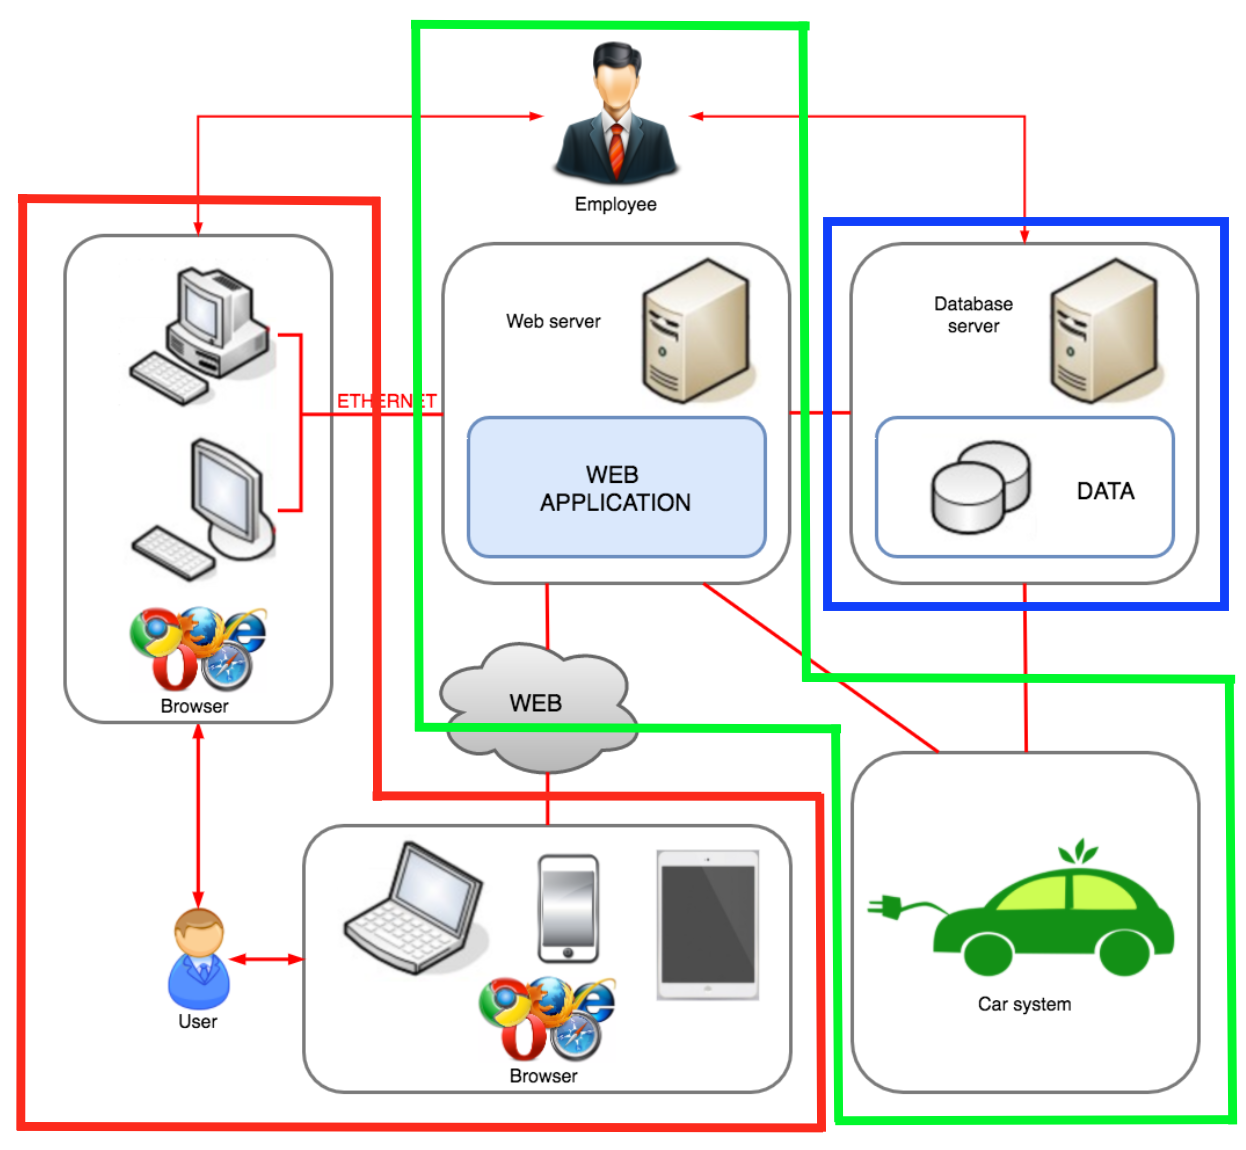
\includegraphics[width=1\textwidth]{General_architecture}
	\caption{General architecture}
\end{figure}
\begin{figure}[H]
	\centering
	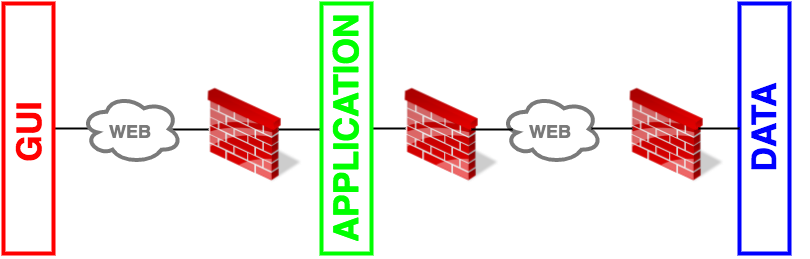
\includegraphics[width=1\textwidth]{3TieredArchitecture}
	\caption{Three-tiered architecture}
\end{figure}
The images represent the main components of our system and show how each component interacts with the others.

The system is based on a three-tiered architecture:
\begin{itemize}
	\item \textbf{Client tier}, which contains web pages (when the users interact with the system through the web application) or an application client (when the users interact with the system through the mobile application).
	\item \textbf{Server tier}, which is divided into two tiers:
	\begin{itemize}
		\item Web tier, which is in charge of generating the web pages and sending them to the client.
		\item Business tier, which contains the application's logic.
	\end{itemize}
	\item \textbf{Database tier}, which contains the database server.
\end{itemize}
\newpage
\begin{figure}[H]
	\centering
	\includegraphics[width=1\textwidth]{HighLevelComponent}
	\caption{High-level architecture}
\end{figure}
The high-level architecture is composed of three different elements.

The client initiates the communication with the server by using the mobile application or the application's website. After making a request, the client has to wait for an answer from the server (synchronous communication). For example, once the client has filled out and submitted the registration form, he has to wait for the server to send him the password via email. 

The server is composed of: 
\begin{itemize}
	\item An employee manager, that will manage the system's information either with a direct access to the database or through the GUI (in this case he will only be able to change the PowerEnJoy cars information).
	\item A ride manager, that will take care of the car management side of our application and will provide an interface to the client.
	\item A user manager, that will provide functions to manage users information and will provide an interface to the client.
	\item A registered user manager, that will provide functions to manage registered users information and will provide an interface to the client.
\end{itemize}

Finally the database, which contains the information about users, cars and reservations, will be accessible by the other three server components.
\newpage 
\subsection{Component view} 
Here the components presented in the previous section are described in details.
\subsubsection{Client component}
The client has three subcomponents:
\begin{enumerate}
	\item \textbf{Client manager}, which possesses all the functionalities related to the generic user, the registered user and the employee. 
	\item \textbf{User interface}, to communicate with the users (registered, not registered and employees).
	\item \textbf{Connection manager}, to communicate with the server.
\end{enumerate}
\begin{figure}[H]
	\centering
	\includegraphics[width=1\textwidth]{ClientComponent}
	\caption{Client component}
\end{figure}
\newpage
\subsubsection{Employee manager component}
The employee manager has four subcomponents:
\begin{enumerate}
	\item \textbf{Connection manager}.
	\item \textbf{Car manager}, that in this case allows the system to change the selected car's information.
	\item \textbf{Account manager}, that provides the login functionalities.
	\item \textbf{Database access component}, used to store persistent data.
\end{enumerate}
\begin{figure}[H]
	\centering
	\includegraphics[width=1\textwidth]{EmployeeComponent}
	\caption{Employee manager component}
\end{figure}
\newpage
\subsubsection{Ride manager component}
The ride manager has seven subcomponents:
\begin{enumerate}
	\item \textbf{Connection manager}.
	\item \textbf{Car manager}, that in this case allows the system to find all the available cars.
	\item \textbf{Reservation manager}, that takes requests from the registered users.
	\item \textbf{Reservation generator}, that creates the reservation after the registered user chooses the car.
	\item \textbf{Database access component}.
	\item \textbf{Notification manager}, that manages the notifications the server needs to send to the client.
	\item \textbf{Email gateway}, manages the sending of emails.
\end{enumerate}
\begin{figure}[H]
	\centering
	\includegraphics[width=1\textwidth]{RideComponent}
	\caption{Ride manager component}
\end{figure}
\newpage
\subsubsection{User manager component}
The user manager has five subcomponents:
\begin{enumerate}
	\item \textbf{Connection manager}.
	\item \textbf{Notification manager}.
	\item \textbf{Email gateway}.
	\item \textbf{Database access component}.
		\item \textbf{Registration manager}, that adds the user's information to the database.
\end{enumerate}
\begin{figure}[H]
	\centering
	\includegraphics[width=1\textwidth]{UserComponent}
	\caption{User manager component}
\end{figure}
\newpage
\subsubsection{Registered user manager component}
The registered user manager has four subcomponents:
\begin{enumerate}
	\item \textbf{Connection manager}.
	\item \textbf{Reservation manager}.
	\item \textbf{Database access component}.
	\item \textbf{Account manager}.
\end{enumerate}
\begin{figure}[H]
	\centering
	\includegraphics[width=1\textwidth]{RegisteredUserComponent}
	\caption{Registered user manager component}
\end{figure}
\subsubsection{Database component}
\begin{figure}[H]
	\centering
	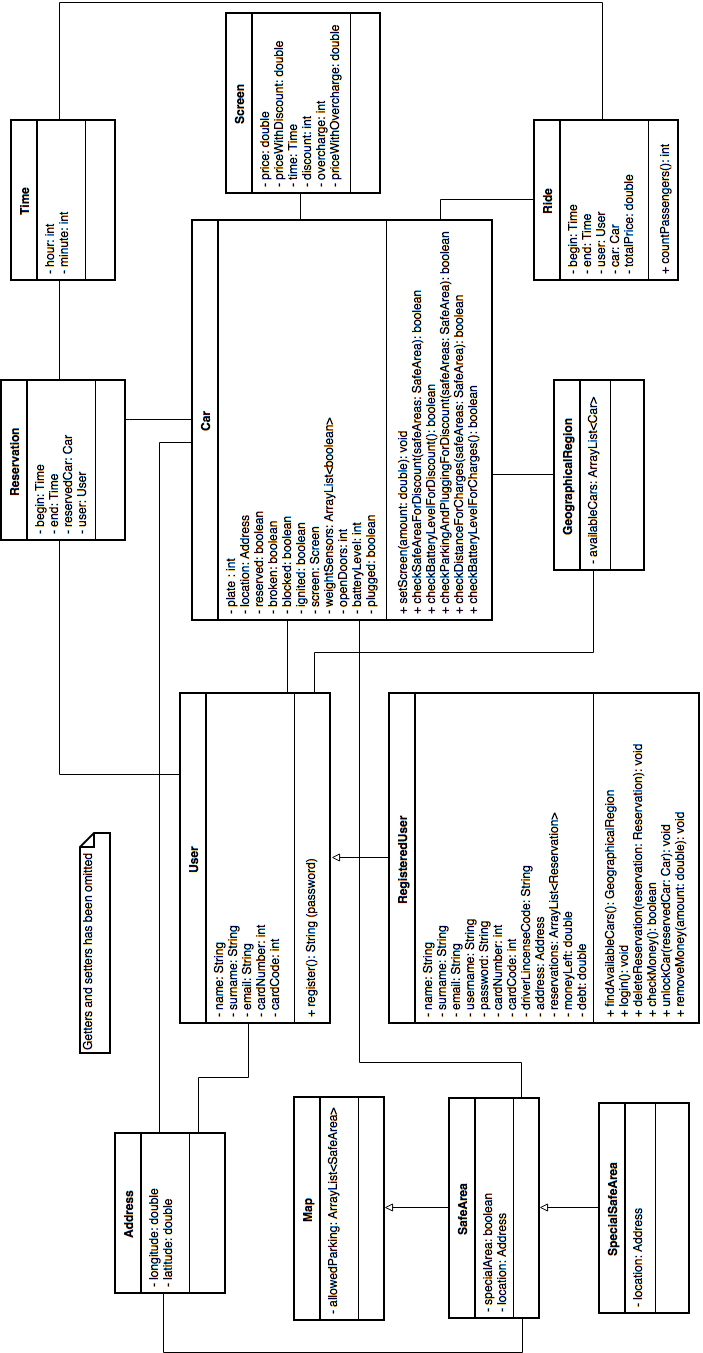
\includegraphics[height=19.5cm]{Class_diagram}
\end{figure}
\subsection{Deployment view} 
The following diagram shows how the whole system will be deployed.
\begin{figure}[H]
	\centering
	\includegraphics[width=1\textwidth]{DeploymentView}
	\caption{Deployment view}
\end{figure} 
\newpage
\subsection{Runtime  view}  
The following sequence diagrams describe the way components interact to accomplish specific tasks related to our use cases.

If the initial action of a diagram corresponds to an already existing sequence diagram, instead of drawing the whole diagram again we thought would be best to just write its name.
\subsubsection{User registration}
 \begin{figure}[H]
 	\centering
 	\includegraphics[width=14cm]{RegistrationSequence}
 \end{figure}
\subsubsection{Registered user and employee login}
\begin{figure}[H]
	\centering
	\includegraphics[width=14cm]{LoginSequence}
\end{figure}
\subsubsection{Registered user views his/her profile}
\begin{figure}[H]
	\centering
	\includegraphics[width=1\textwidth]{ViewProfileSequence}
\end{figure}
\subsubsection{Registered user manages his/her personal information}
\begin{figure}[H]
	\centering
	\includegraphics[width=1\textwidth]{ManagePersonalInfoSequence}
\end{figure}
\subsubsection{Registered user makes a reservation}
\begin{figure}[H]
	\centering
	\includegraphics[width=1\textwidth]{MakeReservationSequence}
\end{figure}
\subsubsection{Registered user reports an issue}
\begin{figure}[H]
	\centering
	\includegraphics[width=1\textwidth]{ReportIssueSequence}
\end{figure}
\subsubsection{Registered user cancels his/her current reservation}
\begin{figure}[H]
	\centering
	\includegraphics[width=1\textwidth]{CancelCurrentReservationSequence}
\end{figure}
\subsubsection{Employee manages a car's information}
\begin{figure}[H]
	\centering
	\includegraphics[width=1\textwidth]{ManageCarInfoEmployeeSequence}
\end{figure}
\newpage
\subsection{Component interfaces} 
This section contains a more detailed description of all the application's interfaces.
\subsubsection{Client interfaces}
\begin{itemize}
	\item \textbf{UIAccess interface}, which provides methods to get user inputs through the user interface.
	\item \textbf{Network interface}, which provides methods to manage the sending and receiving of information with users, server and database.
\end{itemize}
\subsubsection{Employee manager interfaces}
\begin{itemize}
	\item \textbf{User manager interface}, which provides methods through which the client can send a registration request to the server.
	\item \textbf{Registered user manager interface}, which provides methods through which the client can send requests to the server (i.e. login, view profile).
	\item \textbf{Ride manager interface}, provides methods through which the client can send requests to the server (i.e. make a reservation, cancel reservation).
	\item \textbf{Network interface}, which provides methods to manage the sending and receiving of information with users, server and database.
\end{itemize}
\subsubsection{User manager interfaces}
\begin{itemize}
	\item \textbf{Employee manager interface}, which provides methods through which the employee can send requests to the server (i.e. login, manage cars information).
	\item \textbf{Ride manager interface}, provides methods through which the client can send requests to the server (i.e. make a reservation, cancel reservation).
	\item \textbf{Registered user manager interface}, which provides methods through which the client can send requests to the server (i.e. login, view profile).
	\item \textbf{Network interface}, which provides methods to manage the sending and receiving of information with users, server and database.
	\item \textbf{Email gateway interface}, which provides methods to manage the sending and receiving of emails between users and server.
\end{itemize}
\subsubsection{Registered user manager interfaces}
\begin{itemize}
	\item \textbf{Employee manager interface}, which provides methods through which the employee can send requests to the server (i.e. login, manage cars information).
	\item \textbf{User manager interface}, which provides methods through which the client can send a registration request to the server.
	\item \textbf{Ride manager interface}, provides methods through which the client can send requests to the server (i.e. make a reservation, cancel reservation).
	\item \textbf{Network interface}, which provides methods to manage the sending and receiving of information with users, server and database.
\end{itemize}
\subsubsection{Ride manager interfaces}
\begin{itemize}
	\item \textbf{Employee manager interface}, which provides methods through which the employee can send requests to the server (i.e. login, manage cars information).
	\item \textbf{User manager interface}, which provides methods through which the client can send a registration request to the server.
	\item \textbf{Registered user manager interface}, which provides methods through which the client can send requests to the server (i.e. login, view profile).
	\item \textbf{Network interface}, which provides methods to manage the sending and receiving of information with users, server and database.
	\item \textbf{Email gateway interface}, which provides methods to manage the sending and receiving of emails between users and server.
\end{itemize}
\newpage
\subsection{Selected  architectural  styles  and  patterns}
In this section the styles and patterns we used are described.
\subsubsection{Architectural styles}
\begin{itemize}
	\item \textbf{Client-Server}\\
	We have decided to use the Client-Server model because:
	\begin{itemize}
		\item Having centralized control helps to avoid redundancy and conflict issues. It also makes it easier to find files and manage them.
		\item Since all data is stored on the server, it is easy to make a back-up. Also, if data is lost, it can be recovered easily and efficiently.
		\item Scalability.
		\item Accessibility: the server can be accessed remotely by various platforms in the network.
		\item The server can play different roles for different clients.
	\end{itemize}
	\item \textbf{Service-oriented architecture (SOA)}\\
	We have decided to use a service-oriented architecture for the communication between the application server and the client because:
	\begin{itemize}
		\item Flexibility and scalability: possibility to implement the features of the architecture's components in whatever language and platform we choose.
		\item Easier Testing and Debugging: having all the components isolated into various services makes it easier to test and debug all of them individually.
		\item Reusability: since various components are built out separately, it becomes much easier to reuse them later.
	\end{itemize}
	\item \textbf{Three-tiered architecture}\\
	We have decided to use a three-tiered architecture because: 
	\begin{itemize}
		\item It makes the logical separation between business layer, presentation layer and database layer.
		\item As each tier is independent it is possible to enable parallel development of each tier by using different sets of developers.
		\item Easy to maintain.
		\item Since the application layer is a sort of intermediary between the database layer and the presentation layer, the client will not have a direct access to the database, so the database will be safer.
		\item Easy to apply object oriented concepts.
		\item Easy to update data provider queries.
	\end{itemize}
\end{itemize}
\subsubsection{Design patterns}
\begin{itemize}
	\item \textbf{MVC}: we decided to use the Model-View-Controller pattern in order to improve our application. Its main benefits are:
	\begin{itemize}
		\item Makes it easier to reuse the code.
		\item Useful for dividing the work into application control, data structure and data visualization.
		\item Easy to maintain.
		\item Makes it easier for other programmers to understand the code.
		\item Flexible.
	\end{itemize}
\end{itemize}   
\subsection{Other design decisions} 
Since we also need to integrate our mobile and web application with a map service, we decided to use Google Maps.